% ------------------------------------------------------------------------
% ------------------------------------------------------------------------
% ------------------------------------------------------------------------
%                            Trabajo futuro
% ------------------------------------------------------------------------
% ------------------------------------------------------------------------
% ------------------------------------------------------------------------
%\chapter{DISPERSIÓN DE FONONES}

\section{ESTRUCTURA FONÓNICA}

Con el desarrollo de nuevos dispositivos electrónicos se hace indispensable el conocimiento de posibles fases ferroeléctrias para memorias informáticas y dispositivos móviles, incluyendo computación en la nube \cite{Scott2007Ferroelectrics}, ya que la respuesta de la polarización espontánea a excitaciones externas genera efectos físicos como piezoelectricidad, piroelectricidad y propiedades dieléctricas \cite{Shi2016SymmetryFerroelectrics}. En esta sección se discute la dispersión de fonones de las estructuras $Sr_{2}(Ta,Nb)O_{3}N$ para dos ordenamientos aniónicos: \emph{trans-}$Immm(71)$ y \emph{cis-}$Cmcm(63)$ y las fases estables y meta-estables encontradas para estos dos ordenamientos.

\subsection{Relevantes detalles computacionales: Cálculo de estructura fonónica}

El cálculo de estructura fonónica, ó también llamada dispersión de fonones es aplicado ampliamente en materia condensada para el análisis de posibles acoplamientos electrón-fonón ó espín-fonón, y transiciones de fase debido a inestabilidades en la estructura. Lo primero es crear una supercelda de la estructura a investigar, en el presente trabajo se realiza una supercelda $2\times2\times1$ para $Sr_{2}(Ta,Nb)O_{3}N$ \emph{cis-}$Cmcm(63)$ y \emph{trans-}$Immm(71)$. La supercelda no tuvo cambios en dirección [001] debido a la simetría por capas de la estructura, no lo requería. Con la supercelda se procede a hacer el cálculo para encontrar la matriz dinámica, que contiene las constantes de fuerza ínter-atómica, definidas como la segunda derivada de la energía respecto a los desplazamientos atómicos. La imposibilidad de converger este cálculo computacionalmente pesado, con 56 átomos para el orden \emph{trans}, y 112 átomo para el orden \emph{cis}, se establece el método de diferencias finitas donde se desplaza un átomo en una dirección especifica y se calcula cómo responden los átomos vecinos al desplazamiento de fuerzas. Los desplazamientos fueron encontrados mediante el código \textsc{phonopy} \cite{Togo2015phonopy}. Para el ordenamiento aniónico \emph{trans} se obtuvieron 7 desplazamientos, mientras que para el orden de aniones \emph{cis} se obtuvieron 14 desplazamientos, los cuales fueron unidos para generar la matriz constantes de fuerzas interatómicas. Una vez se genera la matriz, se agrega a la celda unitaria, mostrando las curva de dispersión de fonones. Cabe aclarar que en \textsc{phonopy}, las simetrías se buscan con las operaciones de simetría del grupo espacial de la estructura cristalina y comprobando si es invariante después de las operaciones de simetría. En este análisis, se utiliza una tolerancia de distancia $1\times10^{-3}$e en la configuración \emph{cis} para tolerar las pequeña desviaciones de la celda, y el valor predeterminado es $1\times10^{-5}$, el cual fue usado en la configuración \emph{trans}. 

Se agregó una corrección no analítica usando el método Wang \textit{et. al.} \cite{Wang_2010-nac} que usa las constantes de fuerza calculadas en el espacio real y las interacciones dipolo-dipolo calculadas por la teoría de respuesta lineal en el espacio recíproco. La corrección se aplica a la matriz dinámica y se activa con el archivo \textsc{born}, el cual contiene la información de la carga efectiva de Born y la constante dieléctrica \cite{Pick1970Aproximation}. En los cristales polares, surgen campos eléctricos macroscópicos de largo alcance que están asociados con fonones ópticos longitudinales de onda larga. Estos campos eléctricos son el resultado del carácter de largo alcance de la interacción de Coulomb \cite{Baroni2001theory}, y son responsables del conocido fenómeno de división \textsc{lo-to}, es decir, el cambio de frecuencia entre fonones ópticos longitudinales y ópticos transversales en el centro de la zona de Brillouin. Este acoplamiento entre fonones ópticos y campos eléctricos se cuantifica mediante la carga efectiva de Born, que se define mediante:

\begin{equation}
    Z^{\circ}_{\kappa\alpha\beta}=-\frac{\delta^{2}\Vec{E}}{\delta\epsilon_{\beta}\delta\\Vec{u}_{\kappa\alpha}}
    \label{Eq. Born}
\end{equation}

Son el coeficiente de proporcionalidad que relaciona un cambio en la dirección $\alpha$ debido a un campo eléctrico homogéneo aplicado en dirección $\beta$.

\subsection{Configuración con ordenamiento tipo \emph{trans}}

Se presenta la curva de dispersión de fonones de las configuraciones \emph{trans-}$Immm(71)$ de las estructuras $Sr_{2}TaO_{3}N$ y $Sr_{2}NbO_{3}N$ ilustradas en la figura \ref{trans-phon}(a) y \ref{trans-phon}(b), respectivamente.

Para el caso de la configuración \emph{trans-}$Sr_{2}TaO_{3}N$ (figura \ref{trans-phon}(a)), la dispersión de fonones muestra un modo imaginario en el punto $X(0.0,0.5,0.0)$ con frecuencia de $-26.43cm^{-1}$, un modo imaginario en el punto $M(0.5,0.5,0.0)$ con frecuencia de $-97.46cm^{-1}$, y 2 modos imaginarios en el punto $R(0.5,0.5,0.5)$ con frecuencias de $-84.87cm^{-1}$ y $-49.21cm^{-1}$. Para el caso de la configuración \emph{trans-}$Sr_{2}NbO_{3}N$ (figura \ref{trans-phon}(b)) se observan 10 modos imaginarios en la zona de Brillouin: 4 en el punto $\Gamma(0.0,0.0,0.0)$ con frecuencias de $-129.06cm^{-1}$, $-114.48cm^{-1}$, $-92.34cm^{-1}$ y $-91.77cm^{-1}$; y 2 modos imaginarios en cada punto $X(0.0,0.5,0.0)$ con frecuencias de $-56.1016cm^{-1}$ y $-45.29cm^{-1}$; $M(0.5,0.5,0.0)$ con frecuencias de $-110.20cm^{-1}$ y $-44.43cm^{-1}$; y $R(0.5,0.5,0.5)$ con frecuencias de $-97.91cm^{-1}$ y $-70.75cm^{-1}$.

\begin{figure}[h!]
    \centering
    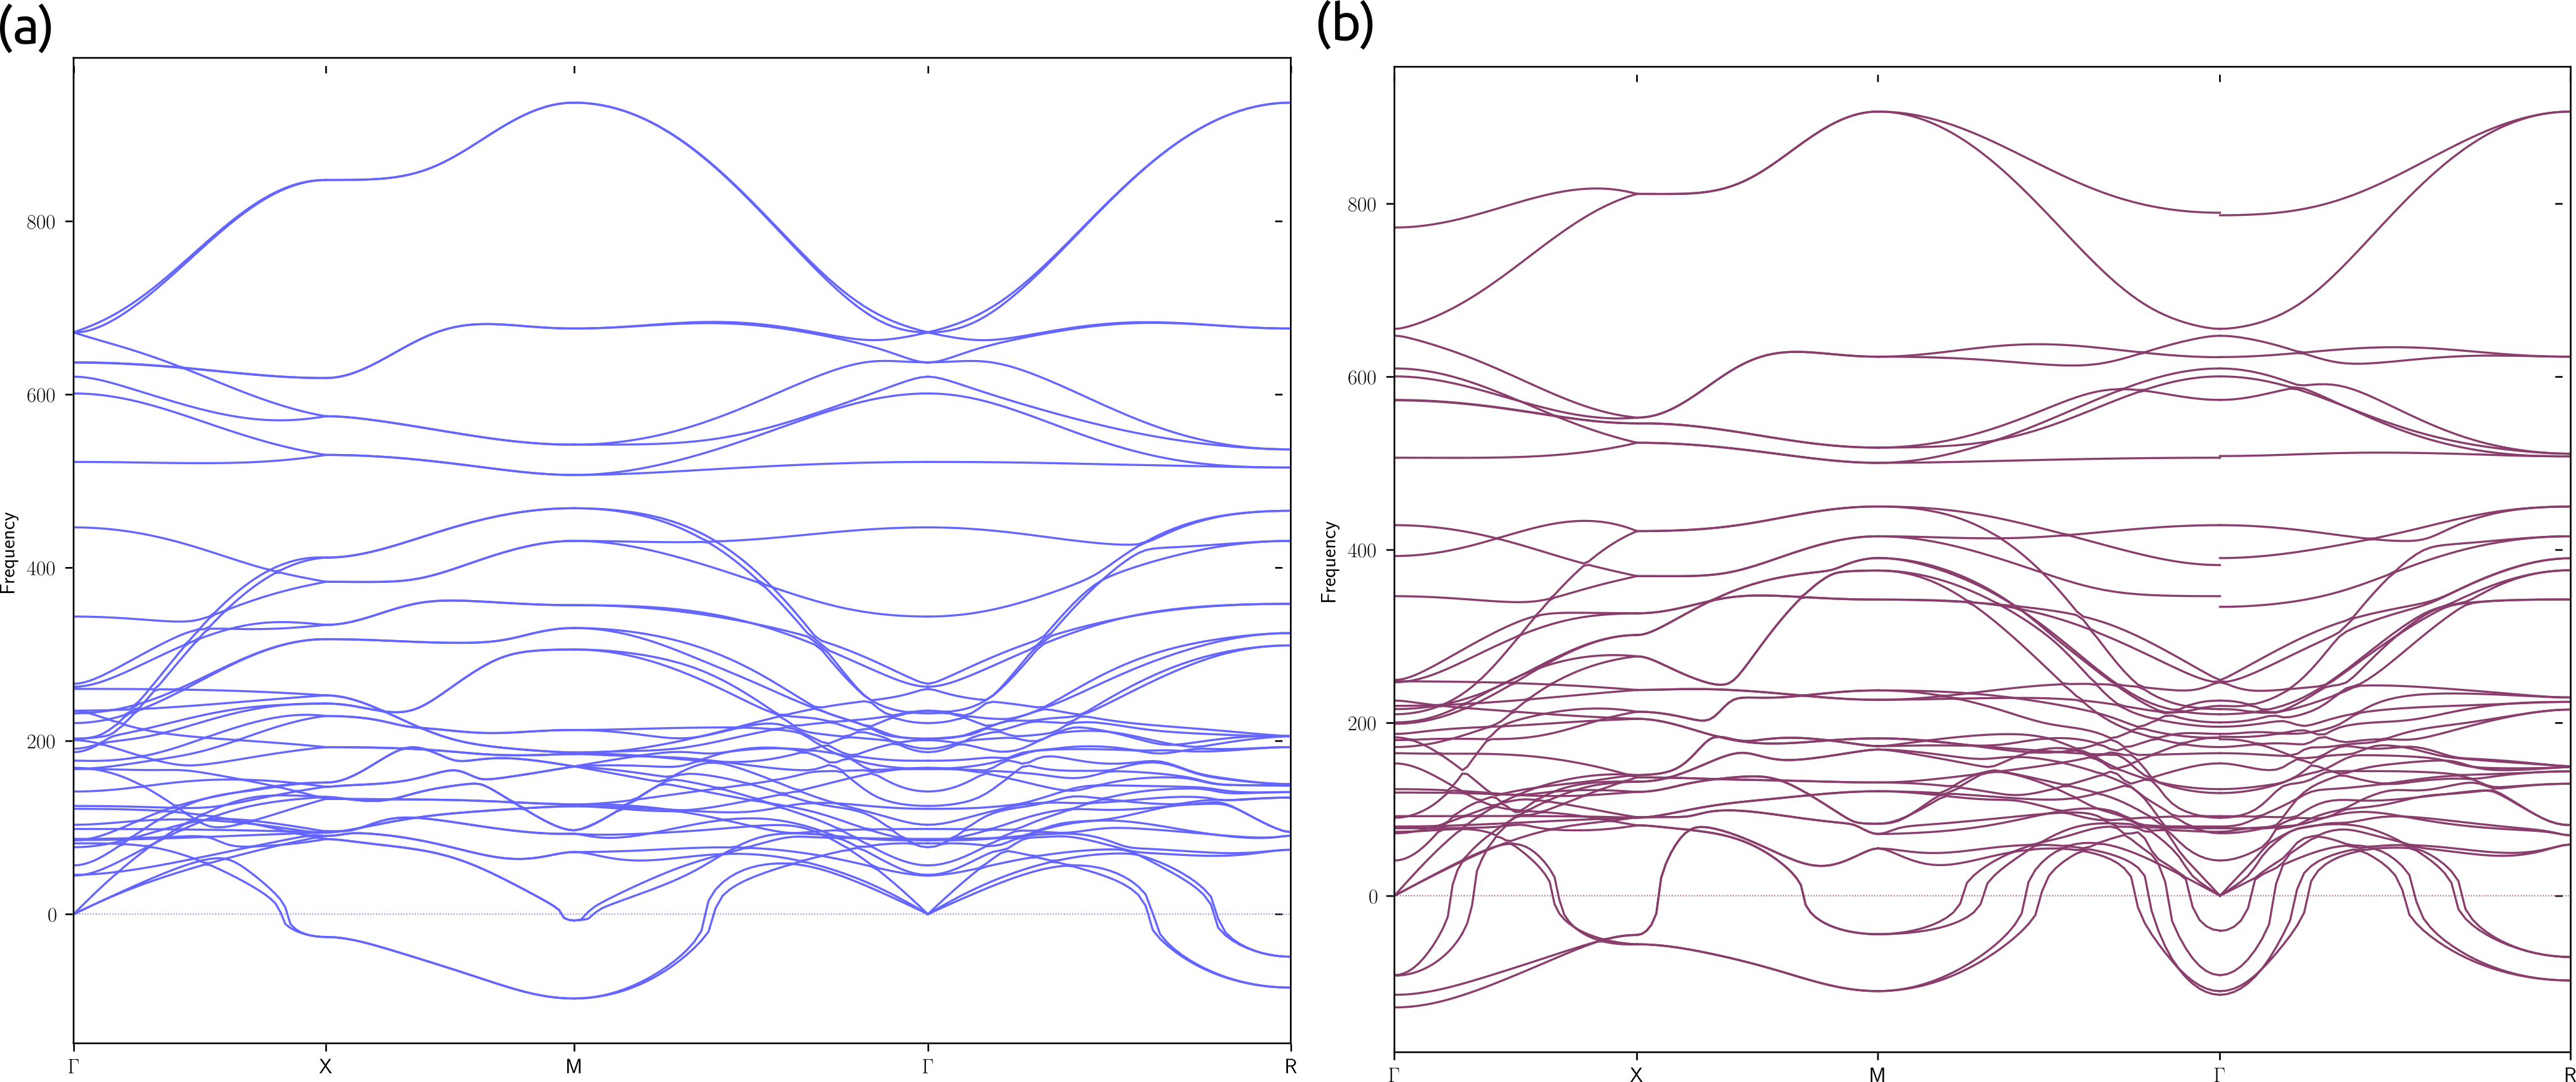
\includegraphics[width=\textwidth]{Figs/dphon-both_trans.png}
    \caption{Dispersión de fonones de la configuración $Immm(71)$ trans (a) $Sr_{2}TaO_{3}N$ y (b) $Sr_{2}NbO_{3}N$.}
    \label{trans-phon}
\end{figure}

Se observa en la dispersión de fonones los 3 modos acústicos que caen en el punto de alta simetría $\Gamma$ de la zona de Brillouin. Esto muestra buenos resultados debido a la corrección no analítica de Wang \cite{Wang_2010-nac} agregada a los cálculos de dispersión de fonones. Sin esta corrección, un modo acústico no cae en el punto $\Gamma$, resultando en solo dos modos acústicos, lo que contradice la teoría de fonones \cite{kaxirasjoannopoulos2019}. Comparando ambas figuras \ref{trans-phon}, se encontró que la estructura $Sr_{2}NbO_{3}N$ tienen modos mas inestables, es decir, de mas baja frecuencia y un numero mayor de modos negativos comparado con la estructura $Sr_{2}TaO_{3}N$. De forma similar sucede en el material tipo perovskita $Sr(Ta,Nb)O_{2}N$ reportado por Gelves \textit{et. al.} \cite{Gelves2021oxynitrides}. Aunque la oxidación en el metal de transición es igual ($Ta^{5+},Nb^{5+}$), la diferencia en los modos inestables puede ser encontrada en la fuerza del enlace entre el metal de transición $(Ta,Nb):5d,4d$ y el nitrógeno $N:2p$, ya que la fuerte interacción covalente conlleva a una ligera mayor repulsión de la nube electrónica, implicando  una mayor inestabilidad de la estructura fonónica \cite{Postnikov1993calculations}. Además, se encontraron modos imaginarios en el punto $\Gamma$ para la estructura $Sr_{2}NbO_{3}N$, lo que no ocurre en la estructura $Sr_{2}TaO_{3}N$.

%no tiene modos imaginarios en el punto de alta simetría $\Gamma$, justamente lo reportado por Gelves \textit{et. al.} \cite{Gelves2021oxynitrides} en la estructura tipo perovskita $SrTaO_{2}N$ 

\subsection{Configuración con ordenamiento tipo \emph{cis}}


Se presenta la curva de dispersión de fonones de las configuraciones \emph{trans-}$Cmcm(63)$ de las estructuras $Sr_{2}TaO_{3}N$ y $Sr_{2}NbO_{3}N$ ilustradas en la figura \ref{cis-phon}(a) y \ref{cis-phon}(b), respectivamente.

\begin{figure}[h!]
    \centering
    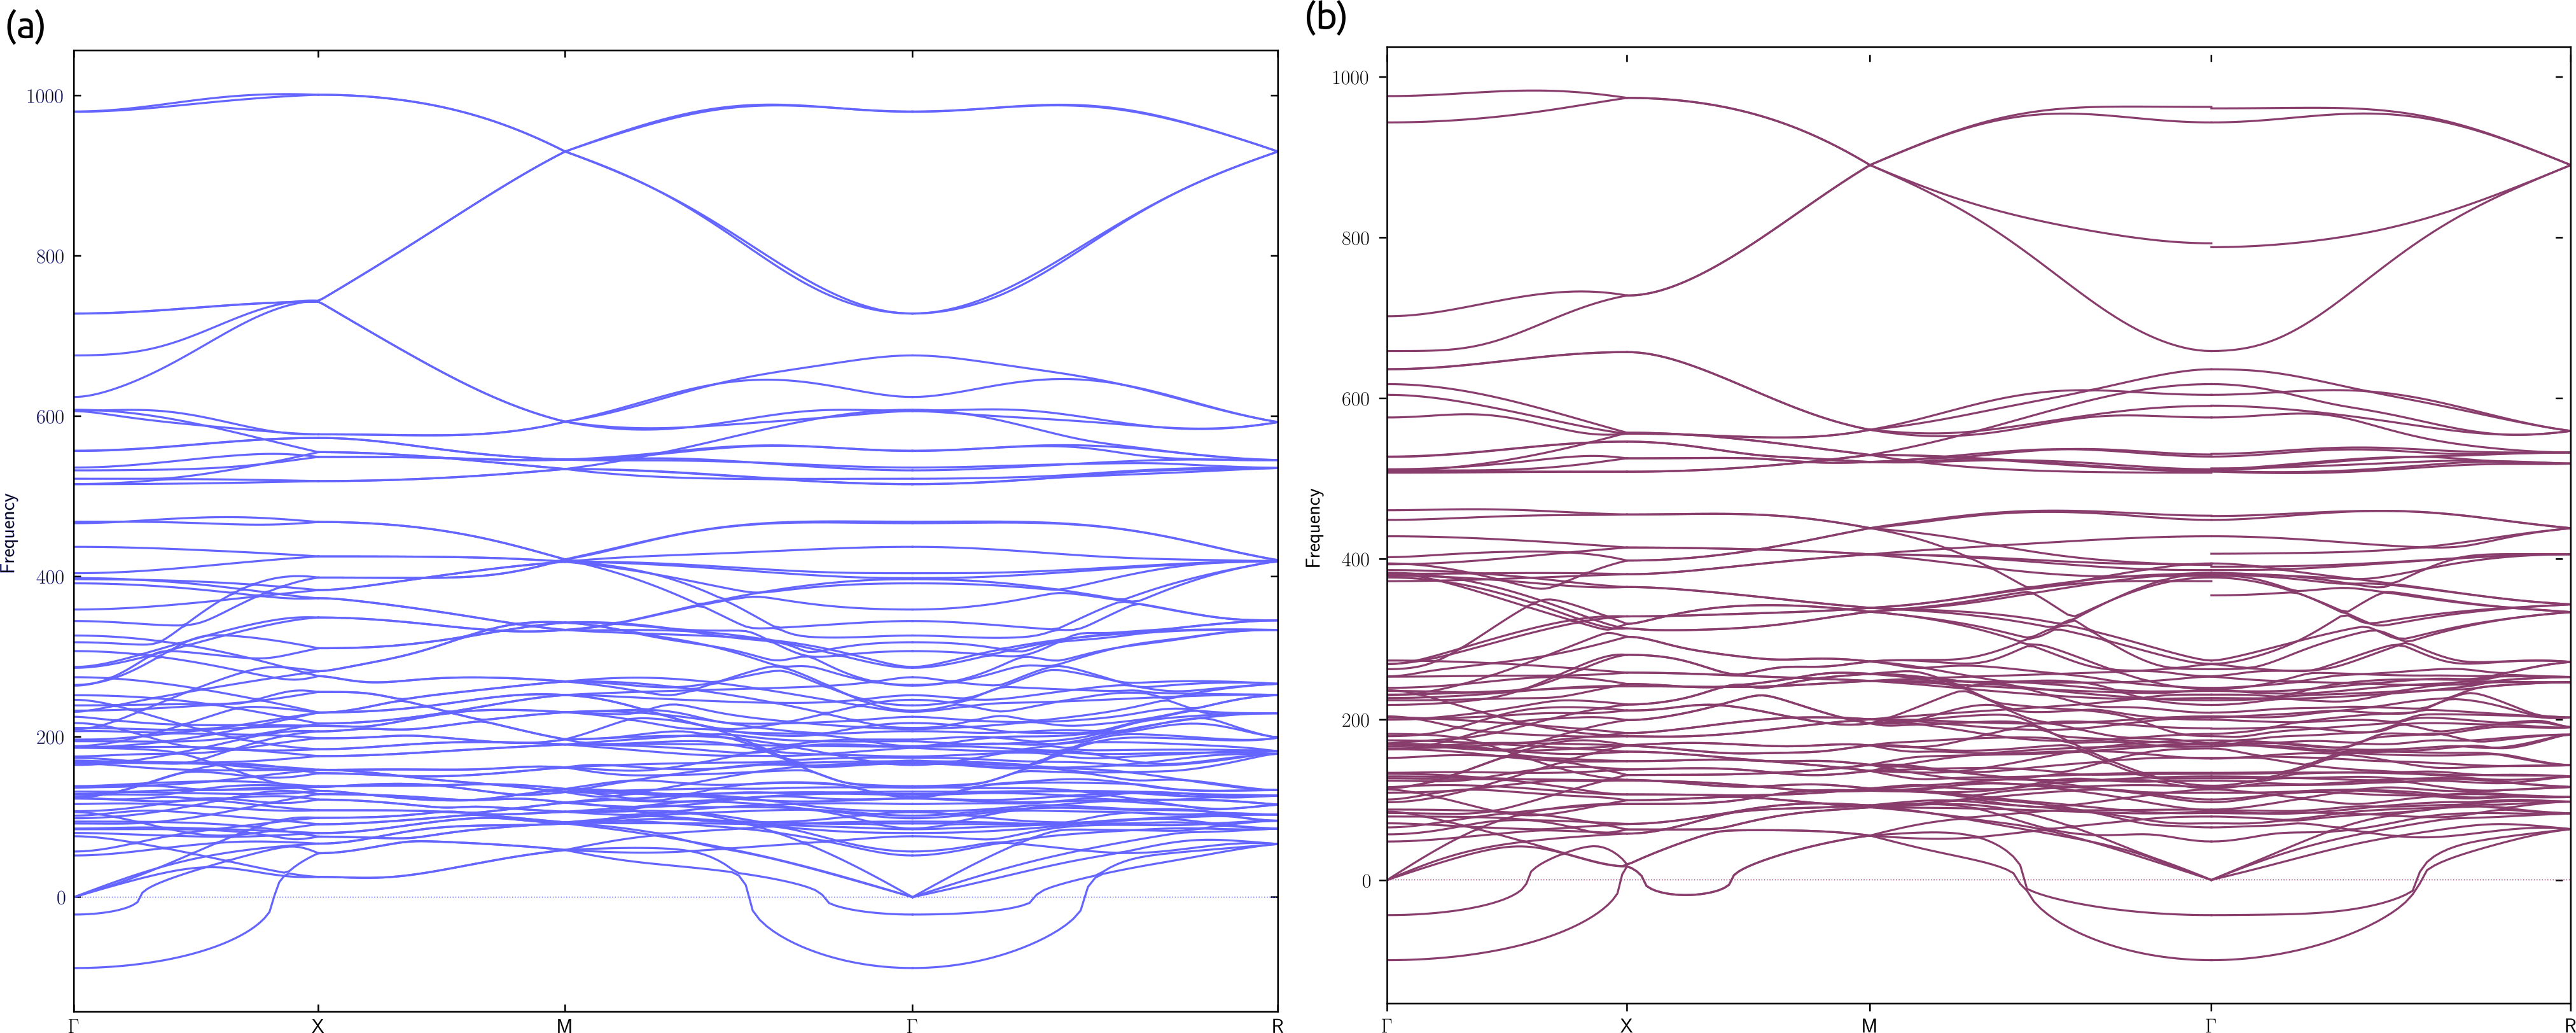
\includegraphics[width=\textwidth]{Figs/dphon-both_cis.png}
    \caption{Dispersión de fonones de la fase $Cmcm(63)$ cis (a) $Sr_{2}TaO_{3}N$ y (b) $Sr_{2}NbO_{3}N$.}
    \label{cis-phon}
\end{figure}

Para el caso de la configuración \emph{cis-}$Sr_{2}TaO_{3}N$ (figura \ref{cis-phon}(a)), la dispersión de fonones muestra 2 modos imaginarios en el punto $\Gamma$ con frecuencias de $-88.45cm^{-1}$ y $-21.74cm^{-1}$. Para el caso de la configuración \emph{cis-}$Sr_{2}NbO_{3}N$ (figura \ref{cis-phon}(b)) se observan 2 modos imaginarios en el punto $\Gamma$ con frecuencias de $-99.93cm^{-1}$ y $-43.86cm^{-1}$. De la misma manera observada en el ordenamiento \emph{trans}, la estructura $Sr_{2}NbO_{3}N$ con orden de aniones \emph{cis} tiene modos imaginarios mas inestables comparados con la estructura $Sr_{2}NbO_{3}N$ con ordenamiento   \emph{cis}. Para este ordenamiento tipo \emph{cis}, solo se encontraron modos imaginarios en el punto de alta simetría $\Gamma$ en la zona de Brillouin, lo que indica un ordenamiento mas estable comparada con la configuración con ordenamiento \emph{trans}. Esto puede deberse a una mas baja energía estructural de la configuración con ordenamiento aniónico \emph{cis} comparado con el ordenamiento aniónico \emph{trans}, como se discutió en el capítulo \ref{Cap. 2}, específicamente en la sección \ref{Sec. 2.2}.

Los modos imaginarios, representados con valores negativos en las figuras \ref{trans-phon} y \ref{cis-phon}, indican inestabilidad estructural a $T=0$, lo que sugiere una ruptura de la simetría en la estructura $Immm(71)$ y $Cmcm(63)$. La estructura puede ser estable con una simetría mas baja o con una celda unitaria diferente. Siguiendo este argumento, los materiales ferroeléctricos son inseparables de la ruptura de la simetría, vienen acompañados de la transición de fase de una estructura centro-simétrica perteneciente a uno de los 32 grupos de punto cristalográfico, a una estructura no centro-simétrica que cae a uno de los 10 grupos de punto ferroeléctrico \cite{Shi2016SymmetryFerroelectrics}. Ahora se puede utilizar la teoría de grupos para explicar la ruptura de simetría causada por distorsiones dadas en la estructura, e identificar si sus combinaciones dan como resultado una simetría polar y luego una posible ferroelectricidad\cite{Yoshida2018HybridPhases}.


\subsection{Diagrama de fases meta-estables para la configuración $Sr_{2}TaO_{3}N$}

Se presenta el diagrama de fases estables y meta-estables para la estructura $Sr_{2}TaO_{3}N$ que contiene los modos inestables encontrados en los ordenamientos \emph{trans} y \emph{cis}. Estos modos imaginarios fueron condensados por el método de \textsc{phonopy} \cite{Togo2015phonopy}, que congela las distorsiones de la estructura encontrando una nueva estructura con menor grupo de simetría. De esta manera se puede analizar las oscilaciones de la nueva estructura encontrada y posteriormente determinar la representación irreducible de cada fonón condensado. La representación irreducible fue encontrada mediante el programa \textsc{amplimodes} \cite{Orobengoa2009amplimodes} para analizar la simetría de las estructuras distorsionadas en base al rompimiento de la simetría de la estructura de alta simetría $Immm(71)$ y $Cmcmc(63)$. 

La figura \ref{Ta-irreps} muestra la diferencia de energía de los modos imaginarios ya condensados comparados con la energía estructural de la configuración principal $Immm(71)$, además de mostrar la representación irreducible de cada modo condensado y las distorsiones (flechas rojas) de la perovskita Ruddlesden-Popper mas estable para cada ordenamiento \emph{trans} y \emph{cis}. De la estructura principal $Sr_{2}TaO_{3}N$ se dividen dos ordenamientos aniónicos \emph{trans} y \emph{cis}, que a su vez se dividen en 5 modos condensados y 2 modos condensados, respectivamente. Se observa que los modos condensados de la configuración con ordenamiento \emph{trans} se posicionan en energía por debajo de la estructura principal $Immm(71)$ y bajan de simetría, encontrando estructuras con grupo espacial $Cmma(67)$, $Pmma(62)$ y $C12/c1(15)$.  El único modo en $X$ tiene grupo espacial $Pmma(62)$ y desplazamiento propio $DT_{4}$. Los modos inestables encontrados en el punto de alta simetría $M$ de la figura \ref{trans-phon}(a) tienen grupo espacial $Cmma(67)$ y representación irreducible $S_{2}^{+}$, incluyendo el modo en $R$ con frecuencia $-49.21cm^{-1}$, pero el otro modo de $R$ tiene grupo espacial $C12/c1(15)$ y desplazamiento propio $T_{2}^{+}$, siendo este el de mas baja energía entre los modos con ordenamiento \emph{trans}, con una diferencia de energía de $-49.4043meV$. Para este modo se ha agregado la estructura cristalográfica a la figura \ref{Ta-irreps}, se aprecian las distorsiones de los octaedros producto de los desplazamientos de los aniones mostrando que los nitrógenos se mueve en sentidos opuestos en dirección [001] con muy poca amplitud de desplazamiento comparado con los oxígenos. Los oxígenos que están en el plano se mueven en sentido opuesto en dirección \emph{'c'}, mientras que los oxígenos del sitio axial se mueven en sentido opuesto sobre el plano en dirección [110].

\begin{figure}[H]
    \centering
    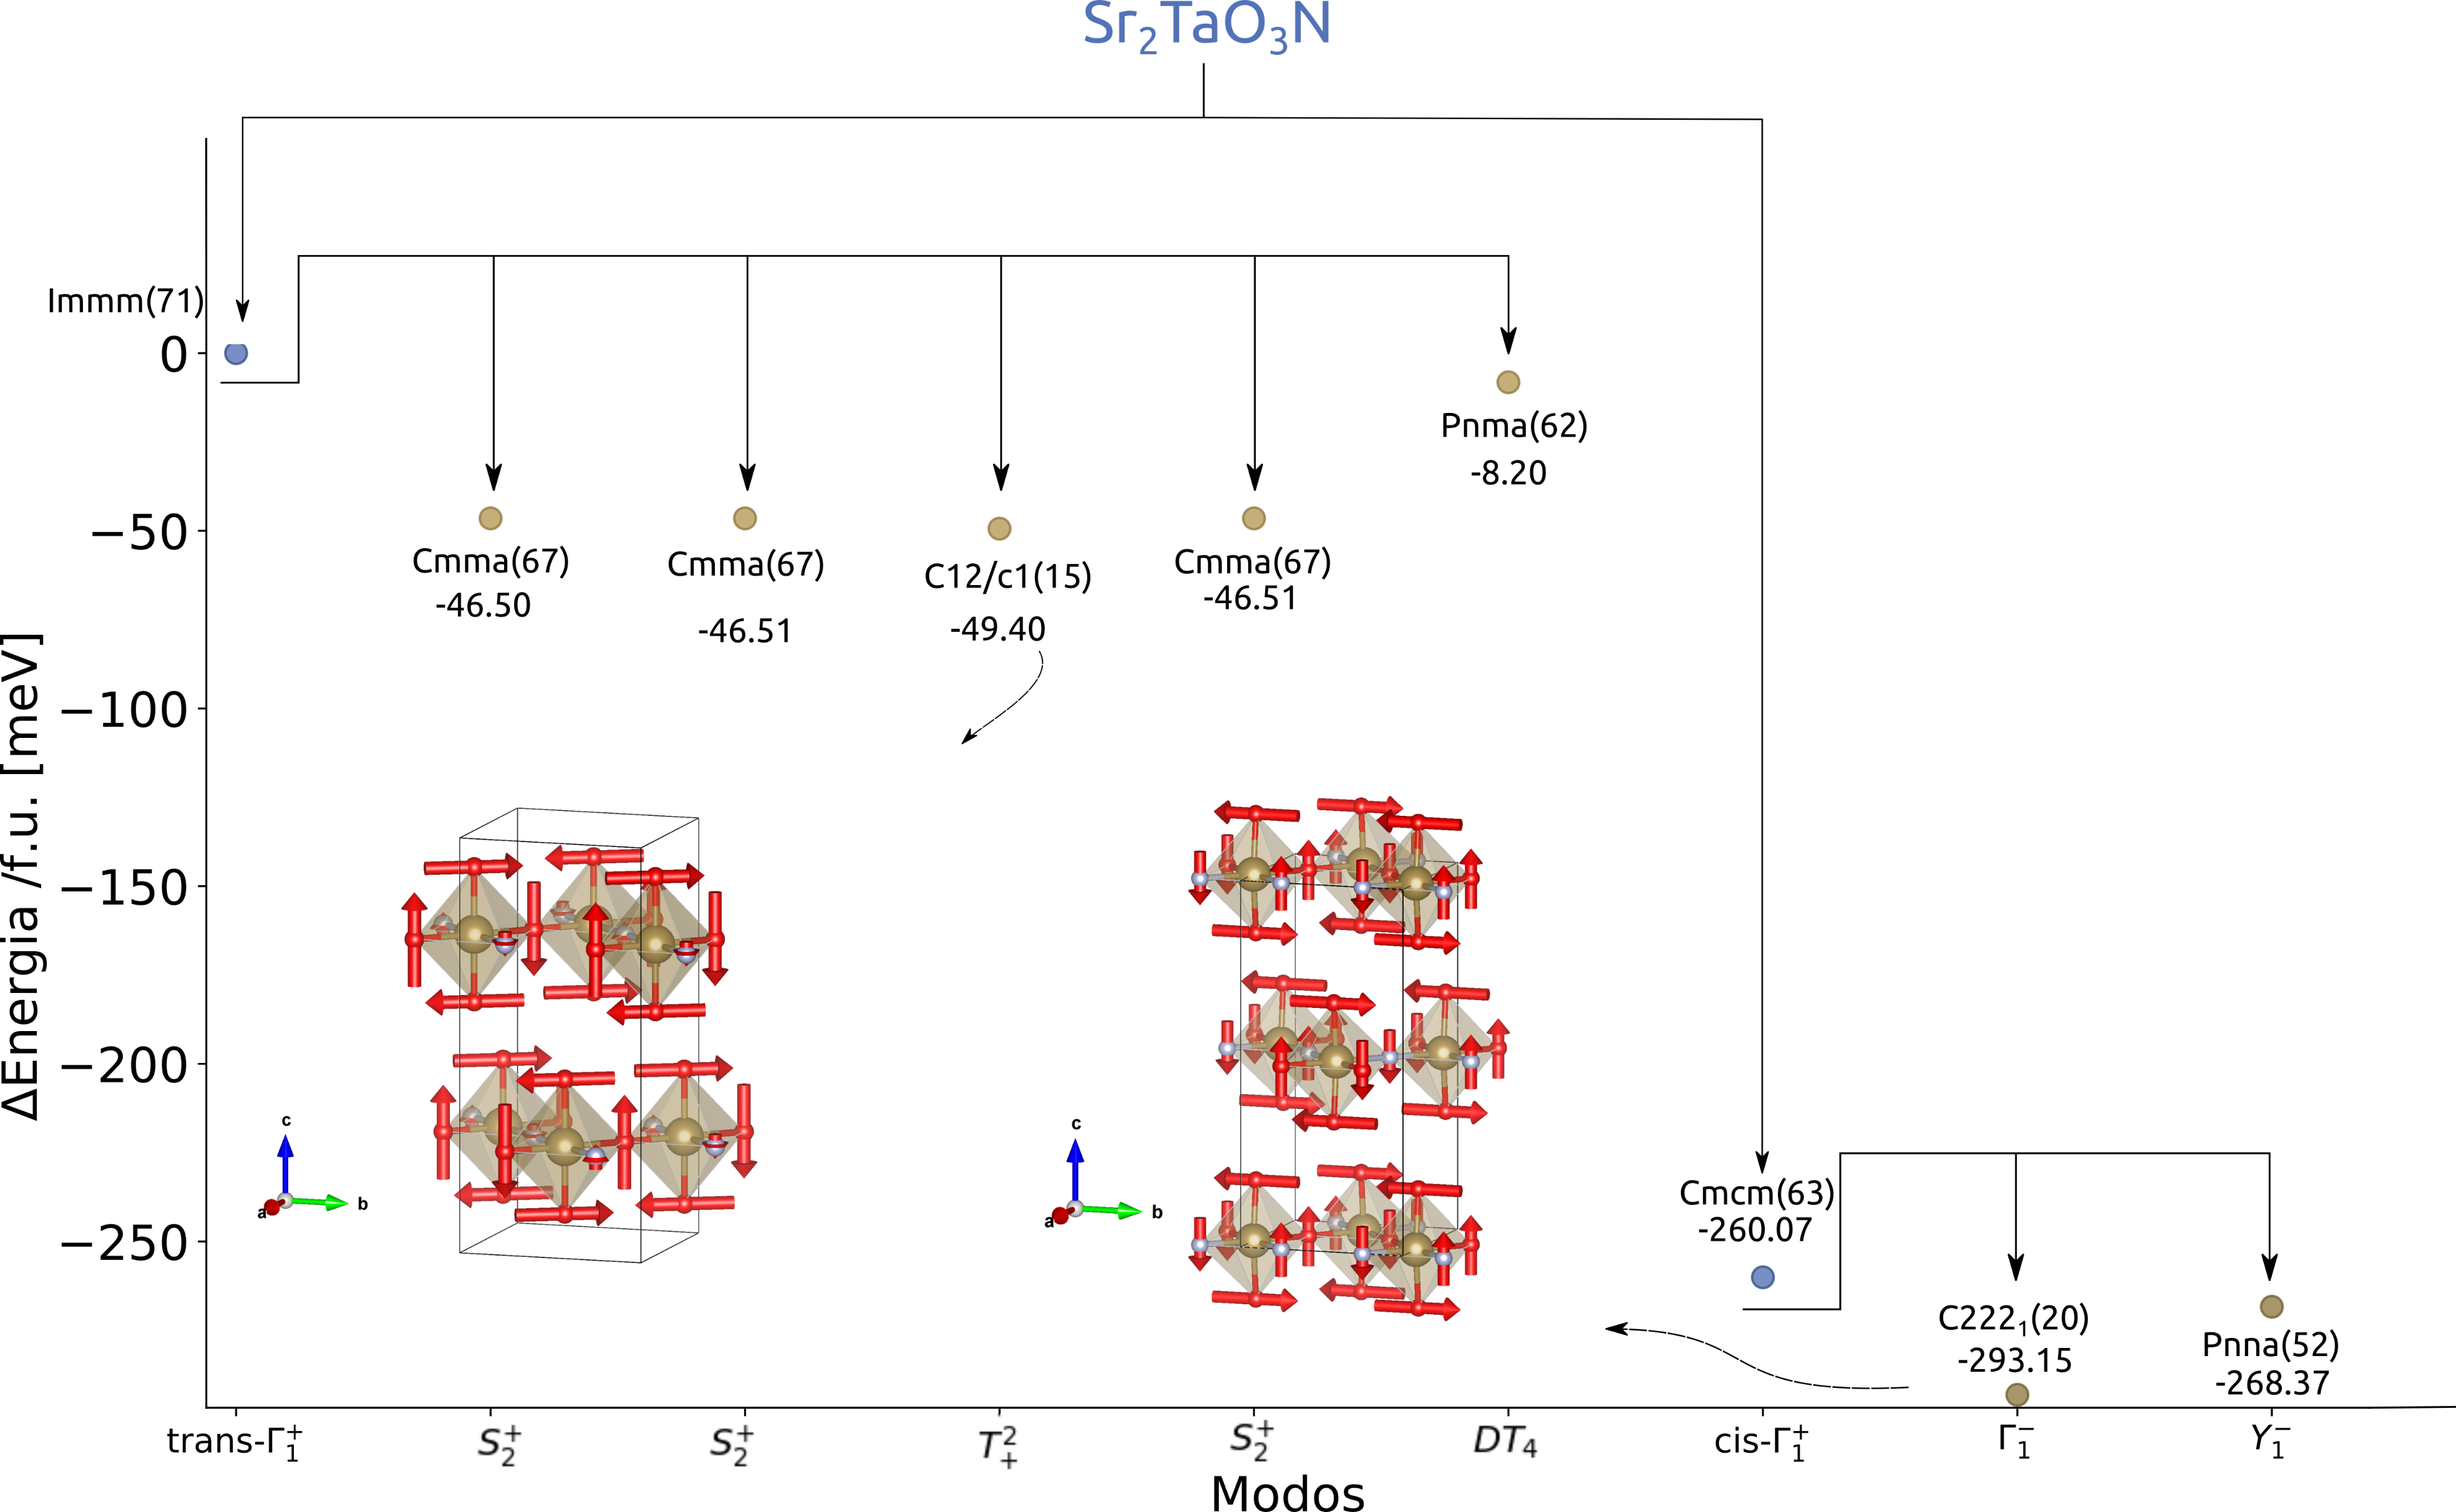
\includegraphics[width=\textwidth]{Figs/Ta-irreps.png}
    \caption{Diagrama de fases meta-estables de $Sr_{2}TaO_{3}N$ para dos principales ordenamientos aniónicos: \emph{trans} y \emph{cis}.}
    \label{Ta-irreps}
\end{figure}

Lo mismo ocurre con los modos condensados de la configuración \emph{cis}, están por debajo en energía y caen a una simetría mas baja que su estructura principal $Cmcm(63)$. La figura \ref{cis-phon}(a) muestra dos modos inestables en $\Gamma$ con grupo espacial $C222_{1}(20)$ y $Pnna(52)$ con desplazamiento propio $\Gamma_{1}^{-}$ y $Y_{1}^{-}$, respectivamente. El modo $\Gamma_{1}^{-}$ es el modo suave encontrado en el diagrama de fases de la estructura $Sr_{2}TaO_{3}N$ (figura \ref{Ta-irreps}),  con una diferencia de energía de $-293.1450meV$. Para este modo se ha agregado la estructura cristalográfica a la figura \ref{Ta-irreps}, se aprecian las distorsiones de los octaedros producto de los desplazamientos de los aniones mostrando que un nitrógeno se mueve en un sentido en dirección [001], el otro nitrógeno se mueve en el sentido opuesto, pero en la misma dirección. Lo mismo sucede con los oxígenos en el plano, mientras que los oxígenos del sitio axial se mueven sobre el plano en sentidos opuesto con una ligera mayor amplitud en los desplazamientos. 

\subsection{Diagrama de fases meta-estables para la configuración $Sr_{2}NbO_{3}N$}

Se presenta el diagrama de fases estables y meta-estables para la estructura $Sr_{2}NbO_{3}N$ que contiene los modos inestables encontrados en los ordenamientos \emph{trans} y \emph{cis}. Asi como en el diagrama de fases de la figura \ref{Ta-irreps}, la figura \ref{Nb-irreps} muestra los modos imaginarios condensados por el método de \textsc{phonopy} \cite{Togo2015phonopy}, la representación irreducible fue encontrada mediante el programa \textsc{amplimodes} \cite{Orobengoa2009amplimodes} para analizar la simetría de las estructuras distorsionadas en base al rompimiento de la simetría de la estructura de alta simetría $Immm(71)$ y $Cmcmc(63)$. 


La figura \ref{Nb-irreps} muestra la diferencia de energía de los modos imaginarios ya condensados comparados con la energía estructural de la configuración principal $Immm(71)$, además de mostrar la representación irreducible de cada modo condensado y las distorsiones (flechas rojas) de la perovskita Ruddlesden-Popper mas estable para cada ordenamiento \emph{trans} y \emph{cis}. De la estructura principal $Sr_{2}NbO_{3}N$ se dividen dos ordenamientos aniónicos \emph{trans} y \emph{cis}, que a su vez se dividen en 10 modos condensados y 2 modos condensados, respectivamente. Se observa que los modos condensados de la configuración con ordenamiento \emph{trans} se posicionan en energía por debajo de la estructura principal $Immm(71)$ y bajan de simetría. Dos modos condensados en $\Gamma$ muestran grupo de simetría $Imm2(44)$ con desplazamiento propio $\Gamma_{2}^{-}$ y $\Gamma_{4}^{-}$, respectivamente; mientras que los otros dos modos $Pmmn(59)$ con desplazamiento propio $X_{2}^{-}$ y $X_{4}^{-}$, respectivamente. Los dos modos encontrados en $X$ muestran grupo de simetría $Pmna(62)$ con desplazamiento propio $DT_{4}$ y $DT_{3}$, respectivamente. Los modos encontrados en $M$ y $R$ muestran el mismo desplazamiento propio $S_{2}^{+}$ con grupo de simetría $Cmma(67)$, $P121(3)$, $P12/c1(13)$ y $C12/c1(15)$. Este ultimo modo es el de mas baja energía entre los modos con ordenamiento \emph{trans}, con una diferencia de energía de $-73.3126meV$. Para este modo se ha agregado la estructura cristalográfica a la figura \ref{Nb-irreps}, se aprecian las distorsiones de los octaedros producto de los desplazamientos de los aniones mostrando que los nitrógenos se mueve en sentidos opuestos en dirección [001] con una mayor amplitud de desplazamiento comparado con los oxígenos. Los oxígenos que están en el plano se mueven en sentido opuesto en dirección [001], mientras que los oxígenos del sitio axial se mueven en sentido opuesto sobre el plano en dirección [110].

\begin{figure}[H]
    \centering
    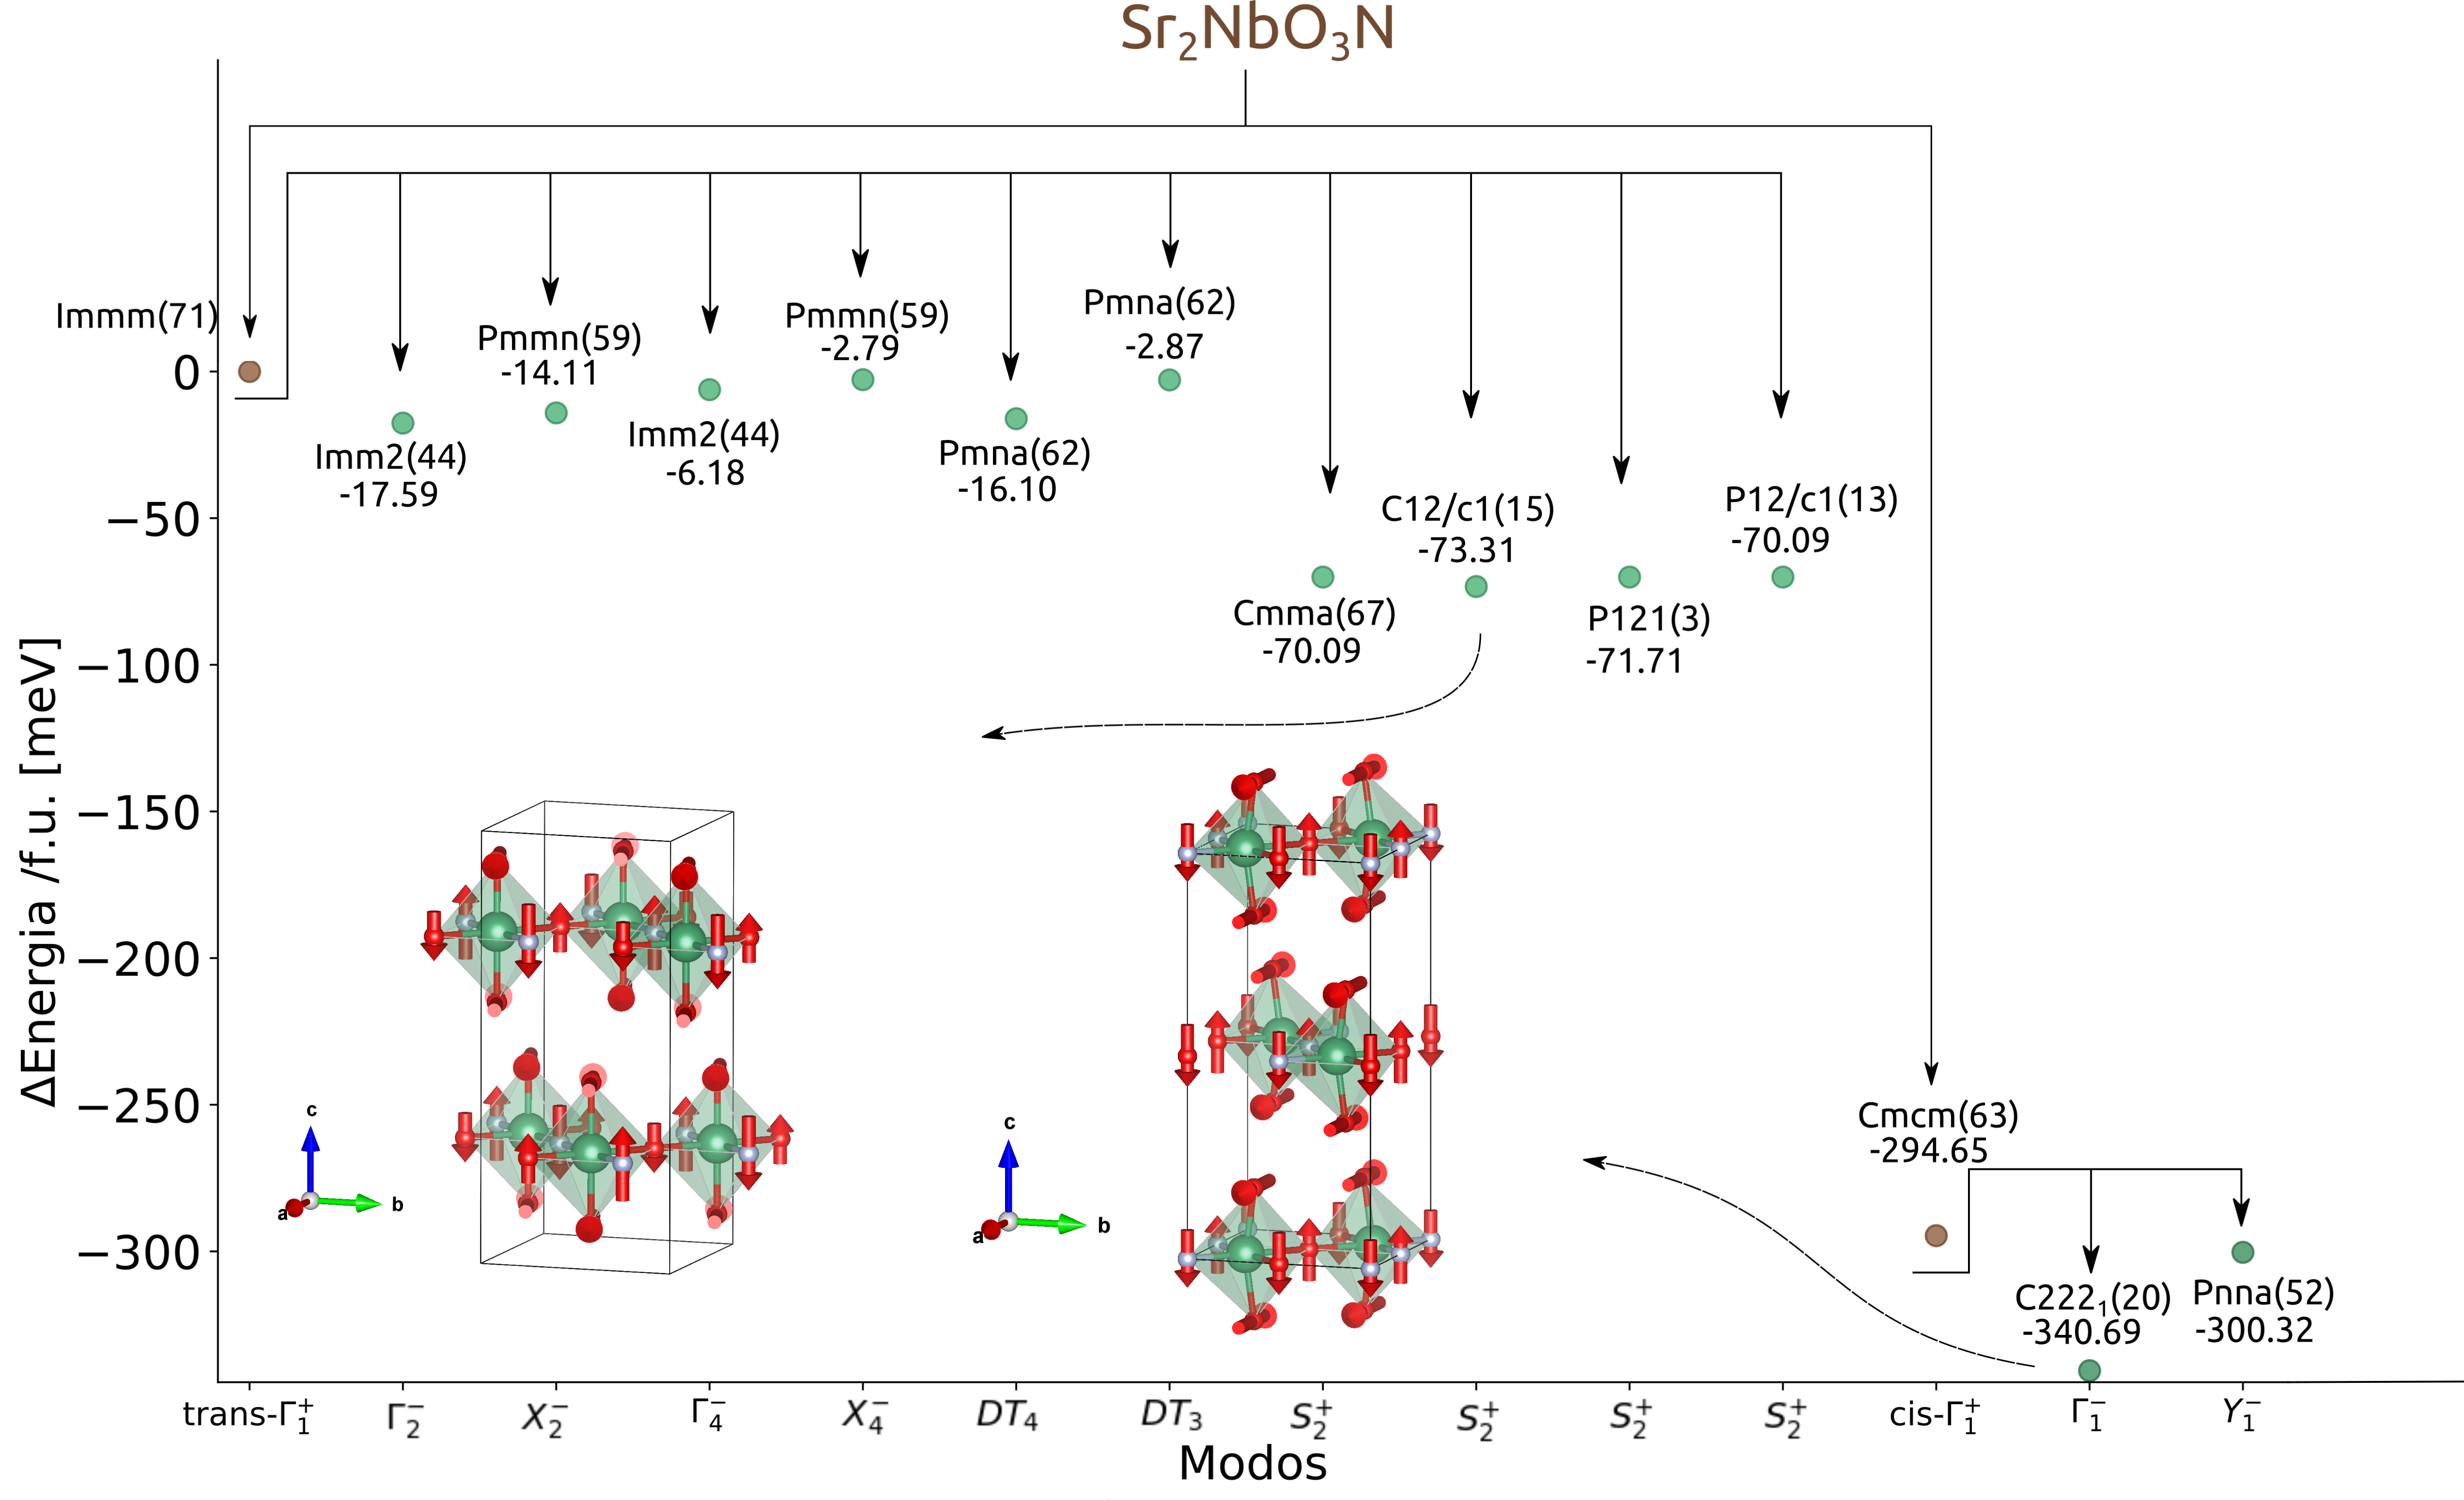
\includegraphics[width=\textwidth]{Figs/Nb-irreps.png}
    \caption{Diagrama de fases meta-estables de $Sr_{2}NbO_{3}N$ de dos principales ordenamientos aniónicos: \emph{trans} y \emph{cis}.}
    \label{Nb-irreps}
\end{figure}

Lo mismo ocurre con los modos condensados de la configuración \emph{cis}, están por debajo en energía y caen a una simetría mas baja que su estructura principal $Ccmmc(63)$. La figura \ref{cis-phon}(b) muestra dos modos inestables en $\Gamma$ con grupo espacial $C222_{1}(20)$ y $Pnna(52)$ con desplazamiento propio $\Gamma_{1}^{-}$ y $Y_{1}^{-}$, respectivamente. El modo $\Gamma_{1}^{-}$ es el modo suave encontrado en el diagrama de fases de la estructura $Sr_{2}NbO_{3}N$ (figura \ref{Nb-irreps}),  con una diferencia de energía de $-340.6840meV$. Para este modo se ha agregado la estructura cristalográfica a la figura \ref{Nb-irreps}, se aprecian las distorsiones de los octaedros producto de los desplazamientos de los aniones mostrando que un nitrógeno se mueve en un sentido en dirección [001], el otro nitrógeno se mueve en el sentido opuesto, pero en la misma dirección. Lo mismo sucede con los oxígenos en el plano, mientras que los oxígenos del sitio axial se mueven sobre el plano en sentidos opuesto. 

Para ambos casos, en las figuras \ref{Ta-irreps} y \ref{Nb-irreps} se observa que la configuración energéticamente mas favorable tiene un orden de aniones \emph{cis} en el plano (ab) y exhibe rotaciones octaédricas tanto en $NbO_{4}N_{2}$ como en $TaO_{4}N_{2}$, lo que esta en concordancia con lo reportado en la literatura \cite{Bouri2018}. La ferroelectricidad puede darse en materiales no-centro-simétricos que pertenezcan a alguno de los 10 grupos de punto polar con dos estados de orientación \cite{Rabe2007ModernFerro}, como lo denota Gelves \textit{et. al.} \cite{Gelves2021oxynitrides} en el doble pozo (ó en inglés \textit{double well}) del material tipo perovskita $Sr(Ta,Nb)O_{2}N$. En este sentido, el modo suave encontrado en ambos materiales tiene el grupo espacial $C222_{1}$ (S.G. 20), el cual pertenece al grupo de punto $222$ según la notación de Herrmann-Mauguin \cite{Hermann2015notation}. En el anexo \ref{anexoC} se aprecian los 10 grupos de punto polar, así que el grupo de punto $222$ no es un material polar. Sin embargo, se ha encontrado que este grupo pertenece al grupo de punto enantiomórfo (ver tabla \ref{Tab. quiral}), lo que indica que el material es un material quiral.






%%%%%%%%%%%%%%%%%%%%%%%%%%%%%%%%%%%% leer para agregar en el marco teorico de phonons    %https://mattermodeling.stackexchange.com/questions/3657/what-do-negative-phonon-frequencies-signify
